\subsection{Limits from LHC@8TeV  and projections for LHC@13TeV}

In this section, we examine limits from the current 8 TeV and projected 13 TeV LHC data. 
We concentrate on limits from mono-jet processes, as these are the mono-object signatures
with the highest cross sections, as shown in Fig.~\ref{fig:cs}.
For mono-jet signals we consider two different processes: $pp\rightarrow h_1h_1j$ and $pp\rightarrow h_1h_2j$.
The cross section of the former depends on the two parameters only, the dark matter mass $M_{h_1}$ and $\lambda_{345}$. 
For the latter, all the vertices depend only on the gauge constants. The only two parameters that shape its cross section 
are the inert scalar masses $M_{h_1}$ and $M_{h_2}$, or equivalently $M_{h_1}$ and $\Delta M = M_{h_2} - M_{h_1}$. 

In order to calculate the limits from the LHC at 8 TeV, we used the {\tt CheckMATE}
\cite{Drees:2013wra,deFavereau:2013fsa,Cacciari:2011ma,Cacciari:2005hq,Cacciari:2008gp,Read:2002hq,Lester:1999tx,Barr:2003rg,Cheng:2008hk} framework, which allows an easy
application of the implemented search analyses. This tool takes a given sample of Monte Carlo events in the HEP or HepMC format after parton showering and hadronisation,
for which we used {\tt Pythia-6} \cite{Sjostrand:2006za}, and performs a detector simulation on these events using Delphes-3 \cite{deFavereau:2013fsa}. Subsequently {\tt CheckMATE} can
apply any of its pre-programmed and validated analyses to the generated signal events and uses the resulting efficiencies along with published information, such as the 95\%
confidence level limit on signal count, to produce results from which we can find the cross-section limit placed on our model by each analysis.

The signature of both processes that we consider, $pp\rightarrow h_1h_1j$  and $pp\rightarrow h_1h_2j$,
is a high-$p_T$ jet and a large missing transverse momentum, $\MET{}$. 
In the case of $pp\rightarrow h_1h_2j$, the $h_2$ will decay via a $h_1$ and a $Z^{(*)}$-boson. When $\Delta M$ is very small, the decay
products of the $Z$ will generally be too soft to be reconstructed in the detector. Therefore in this case $pp\rightarrow h_1h_2j$ will give a mono-jet + $\MET{}$
signature. Using {\tt CheckMATE} and HepMC files created with the i2HDM model implemented in {\tt CalcHEP}, we calculated the limits given by all of the mono-jet +
$\MET{}$ analyses currently implemented in {\tt CheckMATE} \cite{ATLAS:2012zim,Aad:2014nra,Aad:2015zva,Khachatryan:2014rra} (3 ATLAS and 1 CMS analysis).

For both processes considered, we found that the lowest cross section limits for each benchmark point considered were provided by one of the ATLAS mono-jet +
$\MET{}$ analysis \cite{Aad:2015zva}. These are the limits presented in this section. This analysis requires a leading jet with a $p_T > 120$ GeV and $|\eta|
<2.0$, and the leading jet $p_T/\MET > 0.5$. Furthermore, to reduce multijet background where the large $\MET{}$ originating mainly from the jet energy
mismeasurement, we place a requirement on the azimuthal separation $\Delta \phi (\text{jet},p_T^{\text{miss}}) > 1.0$ between the direction of the missing transverse momentum
and that of each jet. A number of different signal regions are considered with increasing $\MET{}$ thresholds from 150 GeV to 700 GeV. Full details are available in
the ATLAS paper \cite{Aad:2015zva}.

In order to project these limits for increased luminosity and to 13 TeV, we use Monte Carlo events to estimate the efficiencies for the signal and background at 13 TeV, which
is a function of $M_{h_1}$ and depends on the best analysis signal region for each mass. We make the assumption that the analysis cuts for 13 TeV data will be the same as for
8 TeV data, which does not take into account improvements in the signal to background ratio which would likely occur with new analysis cuts at 13 TeV. Therefore our projected
limits will be slightly conservative.

\begin{figure}[ht]
\centering
  \subfigure[$M_{h_1}$ vs cross section at 8 TeV .]{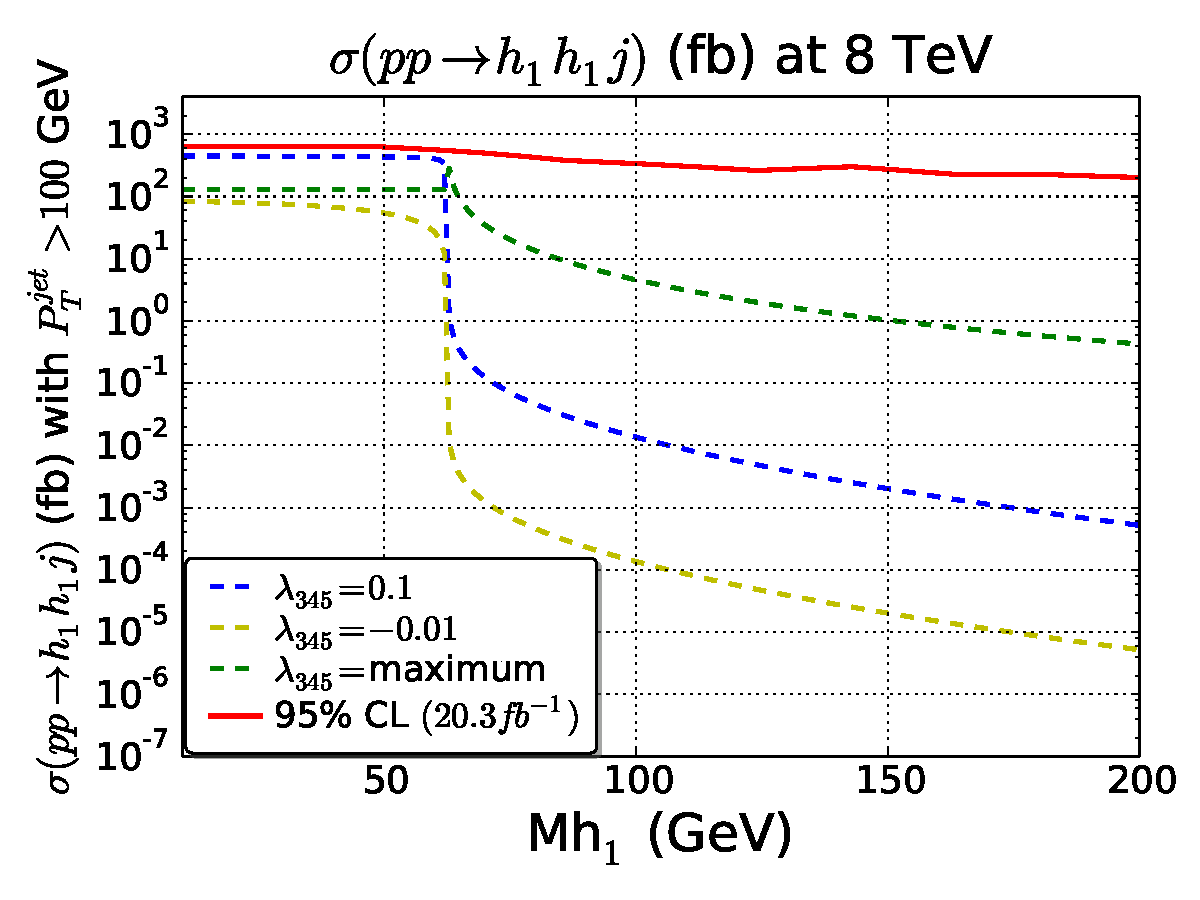
\includegraphics[width=0.5\textwidth]{./Figures/Mh1_h1h1_limit_8TeV.pdf}}%
  \subfigure[$M_{h_1}$ vs cross section at 13 TeV.]{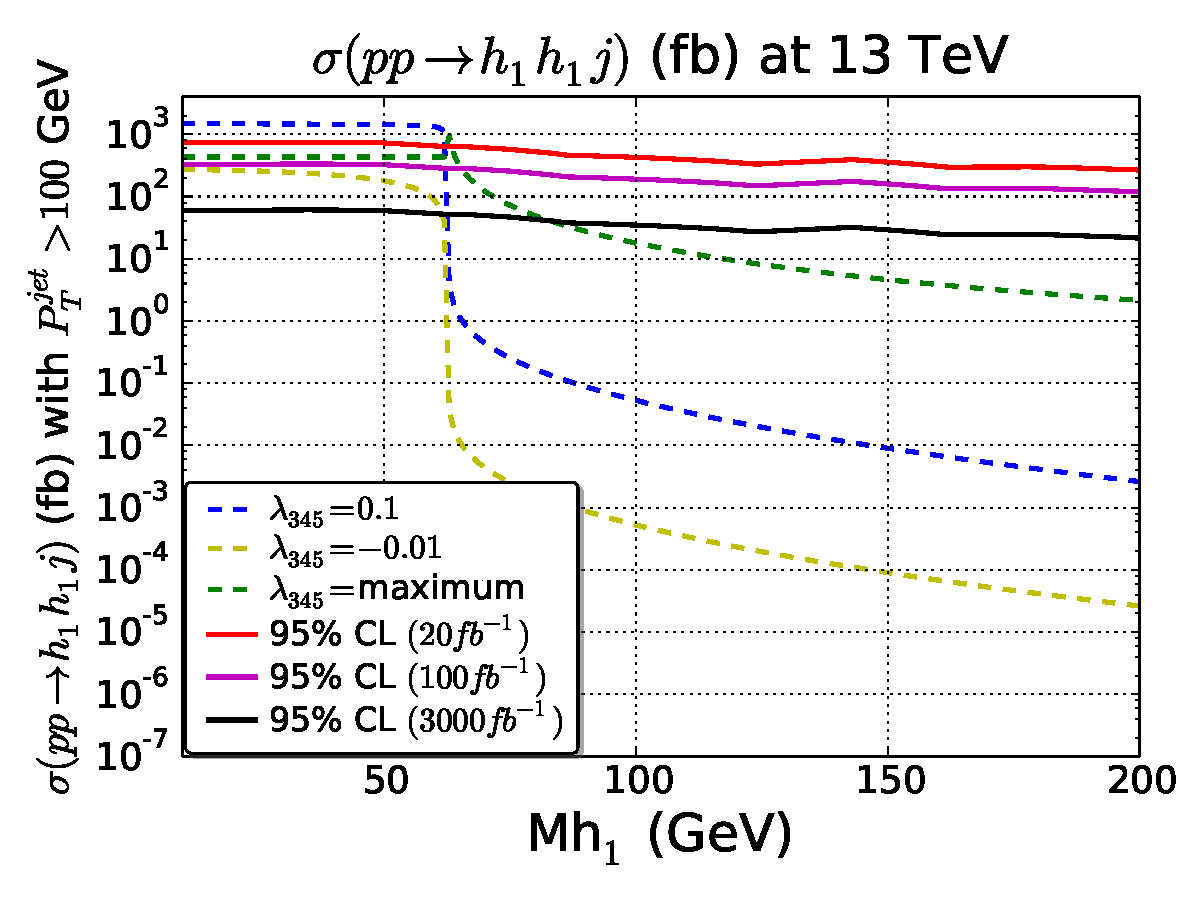
\includegraphics[width=0.5\textwidth]{./Figures/Mh1_h1h1_limit_13TeV.pdf}}
\caption{Cross sections and 95\% CLs for $pp \to h_1 h_1 j$ versus $M_{h_1}$ at 8 TeV and 13 TeV. In both cases, the cross sections are shown for 3 different values of $\lambda_{345}$: (i) $\lambda_{345}=0.1$ ({\bf \blue blue} dashed), (ii) $\lambda_{345}= -0.01$ ({\bf \yellow yellow} dashed), (iii) the maximum $\lambda_{345}$  value ({\bf \green green} dashed) allowed by constraints (described in text). (a) Results for 8 TeV, with limits (solid {\bf \red red}) calculated using the ATLAS analysis \cite{Aad:2015zva}. (b) Results for 13 TeV, with projected limits for the ATLAS analysis \cite{Aad:2015zva} with luminosities of 20 $fb^{-1}$, 100 $fb^{-1}$ and 3000 $fb^{-1}$ ({\bf \red red}, {\bf \magenta magenta}, {\bf black} solid lines) at 13 TeV.} \label{cc_limit_h1h1}
\end{figure}

The results for the process $pp\rightarrow h_1h_1 j$ are shown for 8 TeV in Fig.~\ref{cc_limit_h1h1} (a) with projections to 13 TeV and higher luminosities in Fig.~\ref{cc_limit_h1h1} (b). The limits are denoted by the solid lines, whilst the cross sections for the i2HDM for different values of $\lambda_{345}$ are shown by the dashed lines. For $M_{h_1} < M_H/2$, the maximum allowed value of $\lambda_{345}$ is given by the bound on the invisible Higgs branching ratio in Eq.~(\ref{eq:lhc-higgs-invis}) (this constraint has not been applied on the dashed blue $\lambda_{345} = 0.1$ curve), whilst when $M_{h_1} > M_H/2$ the maximum allowed value is calculated using the constraints of Eq.~(\ref{eq:l345-vacuum-stab}). The cross section with this maximum value of $\lambda_{345}$ is denoted by the dashed green line. We see in Fig.~\ref{cc_limit_h1h1} (a), that the 8 TeV LHC mono-jet + $\MET{}$ searches do not constrain the i2HDM via the $pp\rightarrow h_1h_1 j$ process. However at 13 TeV, shown in Fig.~\ref{cc_limit_h1h1} (b), with around 100 $fb^{-1}$ of data (purple solid), we would be able to set limits on $\lambda_{345}$ for $M_{h_1}$ up to 66 GeV, and for 3000 $fb^{-1} $ (black solid) LHC data would set limits on $\lambda_{345}$ for $M_{h_1}$ up to 83 GeV. 
It should be remarked that the spike in cross section on the green dashed line at $M_{h_1} \sim M_H/2$ is due to the release of the ($H \to invisible$) bound on $\lambda_{345}$ once the decay of the Higgs into DM is kinematically closed.

%It should be explained that the ``spike'' at around  $M_{h_1} \approx 62.5$ GeV for the maximum value of $\lambda_{345}$ (green dashed line) at both 8 and 13 TeV  occurs because when $M_{h_1} < 62.5$ GeV, the Higgs is able to decay via $H \to h_1 h_1$, and the branching ratio is limited to 0.28. However when $M_{h_1}$ is just above 62.5, this decay is closed and there is no constraint on the branching in this scattering process, which can be much larger than 0.28 when $\lambda_{345}$ is at its maximum allowed value. 
\begin{figure}[ht]
\centering
 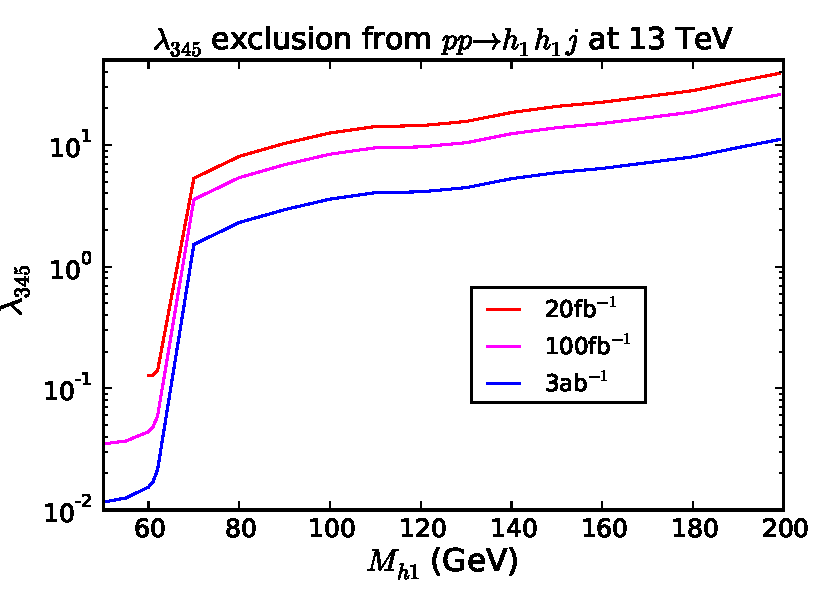
\includegraphics[width=0.65\textwidth]{./Figures/lam345_limit_lhc13.pdf}
\caption{The limit on $\lambda_{345}$ from  $pp \to h_1 h_1 j$ at 13 TeV
derived from the analysis presented in Fig.~\ref{cc_limit_h1h1} \label{lam345_coll_limit}}
\end{figure}

We should note that a similar projection of CMS mono-jet limits \cite{Khachatryan:2014rra} at 14 TeV has been studied previously \cite{Arhrib:2013ela}, where the projected limits were slightly stronger than in Fig.~\ref{cc_limit_h1h1} (b). Their projection was able to limit $M_{h_1}$ for values of $\lambda_{345}$ as small as $\lambda_{345} = 0.01$, while we require slightly larger values of $\lambda_{345}$ in order to limit $M_{h_1}$. 
We would like to note that in our paper the limits are based on the fast detector simulations rather than parton level 
ones used in \cite{Arhrib:2013ela} done for  14 TeV. Taking this into account we consider our results as more realistic
projection of the future LHC data potential.
In Fig.~\ref{lam345_coll_limit} we provide the  limit on $\lambda_{345}$ versus $M_{h_1}$ for different projected luminosities at the LHC@13TeV. This limit is derived from the analysis presented in Fig.~\ref{cc_limit_h1h1} and could be more practical 
for comparison with limits on $\lambda_{345}$ from different experiments.



\begin{figure}[ht]
\centering
  \subfigure[$M_{h_1}$ vs cross section at 8 TeV. ]{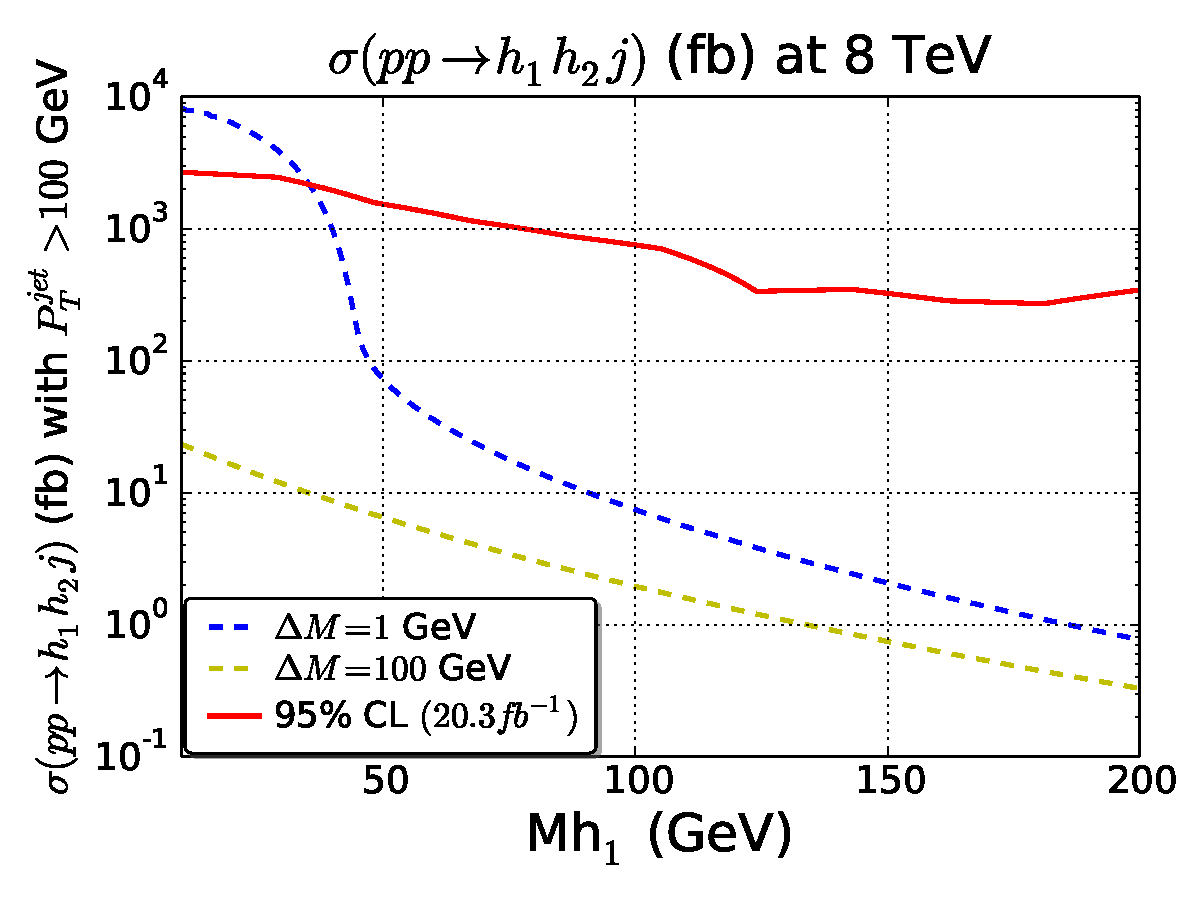
\includegraphics[width=0.5\textwidth]{./Figures/Mh1_h1h2_limit_8TeV.pdf}}%
  \subfigure[$M_{h_1}$ vs cross section at 13 TeV.]{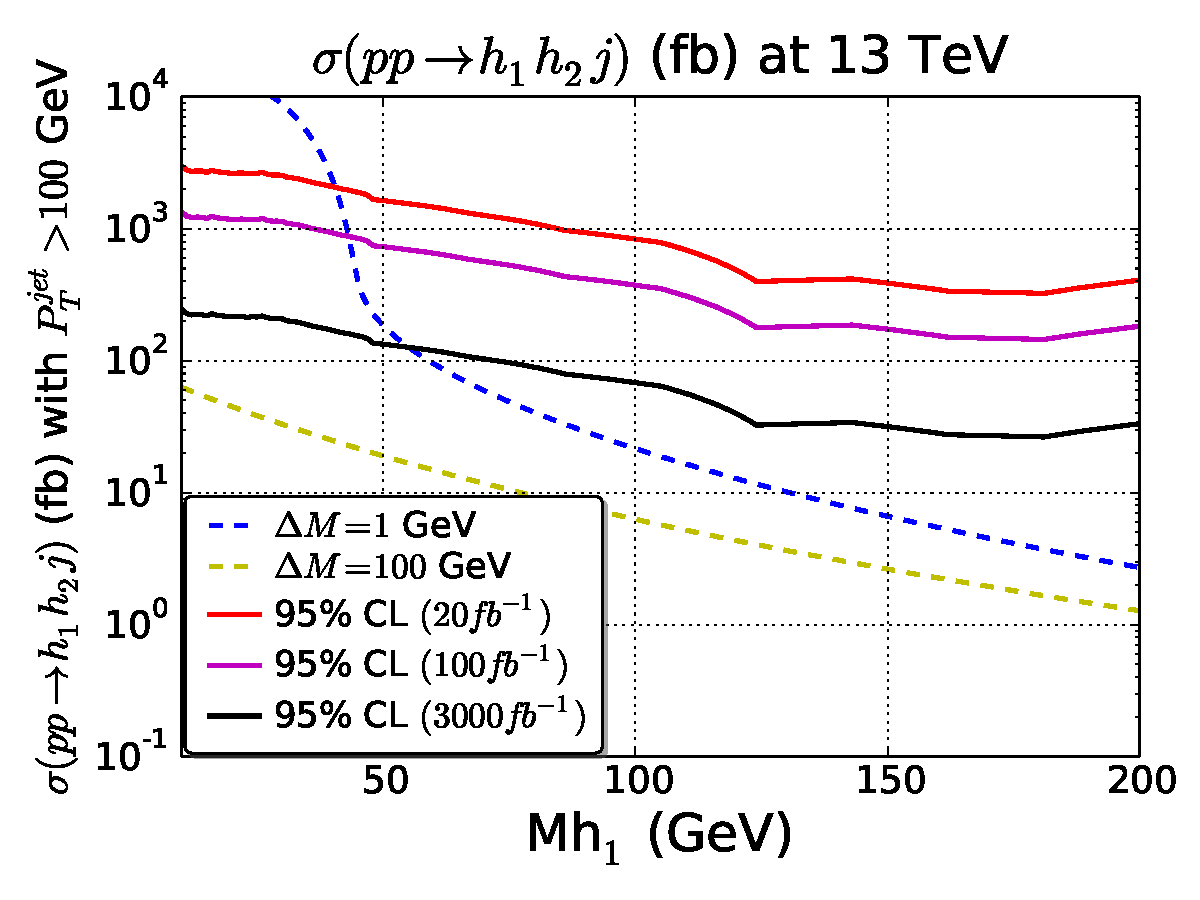
\includegraphics[width=0.5\textwidth]{./Figures/Mh1_h1h2_limit_13TeV.pdf}}
\caption{Cross sections and 95\% CLs for $pp \to h_1 h_2 j$ versus $M_{h_1}$ at 8 TeV and 13 TeV. In both cases, the cross sections are shown for 2 different values of $\Delta M = M_{h_2} - M_{h_1}$: (i) $\Delta M = 1$ GeV ({\bf \blue blue} dashed), (ii) $\Delta M = 100$ ({\bf \yellow yellow} dashed). (a) Results for 8 TeV, with limits (solid {\bf \red red}) calculated using the ATLAS analysis \cite{Aad:2015zva}. (b) Results for 13 TeV, with projected limits for the ATLAS analysis \cite{Aad:2015zva} with luminosities of 20 $fb^{-1}$, 100 $fb^{-1}$ and 3000 $fb^{-1}$ ({\bf \red red}, {\bf \magenta magenta}, {\bf black} solid lines) at 13 TeV.} \label{cc_limit_h1h2}
\end{figure}

For $pp\rightarrow h_1h_2 j$, the results are shown in Fig.~\ref{cc_limit_h1h2}(a) for 8 TeV and in Fig.~\ref{cc_limit_h1h2}(b) for 13 TeV. We consider two scenarios with a small ($\Delta M =1$ GeV in blue) and large ($\Delta M =100$ GeV in yellow) mass split. The projected cross section limits are again denoted by the solid lines. When $\Delta M = 1$ GeV, the current LHC Run I results are able to rule out $M_{h_1} < 35$ GeV. In this case, it should be emphasised that as the couplings of the relevant diagrams (see Fig.~\ref{fig:fd-monojet2}) are fixed by the gauge couplings, this limit on $M_{h_1}$ is independent of all parameters other than $\Delta M$. At 13 TeV, and at higher luminosities, this lower limit on $M_{h_1}$ in this degenerate mass scenario is improved slightly to 41 GeV, 43 GeV and 55 GeV for $20$ fb$^{-1}$ (solid red), $100$ fb$^{-1}$ (solid magenta) and $3000$ fb$^{-1}$ (solid black) of integrated luminosity respectively, as is shown in Fig.~\ref{cc_limit_h1h2} (b). For $\Delta M = 100$ GeV, the production cross section is much smaller and the model is not constrained via mono-jet and $\MET{}$ signatures from the $pp\rightarrow h_1h_2 j$ process. However, in this region other collider signatures such as dilepton + $\MET{}$ from the decay $h_2 \to h_1Z$ are available and will provide stronger limits as studied for example in \cite{Belanger:2015kga}.


%\begin{figure}[ht]
%\centering
%  \includegraphics[width=0.5\textwidth]{./Figures/Mh1_ld345_Omega_large-coll.pdf}%
%  \includegraphics[width=0.5\textwidth]{./Figures/Mh1_Mhc_Omega_large-coll.pdf}\\
%   \includegraphics[width=0.5\textwidth]{./Figures/Mh1_Mh2_Omega_large-coll.pdf}%
%  \includegraphics[width=0.5\textwidth]{./Figures/Mhc_Mh2_Omega_large-coll.pdf}\\
%\caption{}
%\label{}
%\end{figure}


%\begin{figure}[ht]
%\centering
%  \includegraphics[width=0.5\textwidth]{./Figures/Mh1_ld345_Omega_small-coll_zoom.pdf}
%\caption{}
%\label{}
%\end{figure}

%\begin{figure}[ht]
%\centering
%  \includegraphics[width=0.5\textwidth]{./Figures/Mh1_ld345_Omega_small-coll.pdf}%
%  \includegraphics[width=0.5\textwidth]{./Figures/Mh1_Mhc_Omega_small-coll.pdf}\\
%   \includegraphics[width=0.5\textwidth]{./Figures/Mh1_Mh2_Omega_small-coll.pdf}%
%  \includegraphics[width=0.5\textwidth]{./Figures/Mhc_Mh2_Omega_small-coll.pdf}\\
%\caption{}
%\label{}
%\end{figure}

%\begin{figure}[ht]
%\centering
%  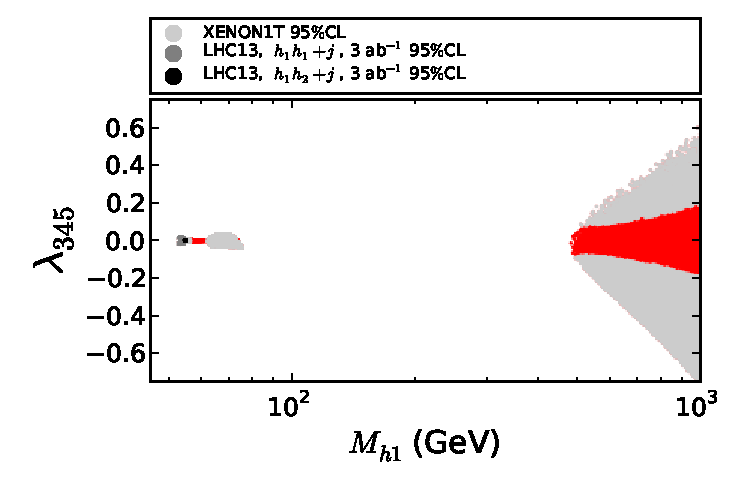
\includegraphics[width=0.5\textwidth]{./Figures/Mh1_ld345_Omega_relic-large-coll_zz-large-monoc.pdf}%
%  \includegraphics[width=0.5\textwidth]{./Figures/Mh1_Mhc_Omega_relic-large-coll_zz-large-monoc.pdf}\\
%  \includegraphics[width=0.5\textwidth]{./Figures/Mh1_Mh2_Omega_relic-large-coll_zz-large-monoc.pdf}%
%  \includegraphics[width=0.5\textwidth]{./Figures/Mhc_Mh2_Omega_relic-large-coll_zz-large-monoc.pdf}\\
%\caption{}
%\label{}
%\end{figure}
%\begin{figure}[ht]
%\centering
%  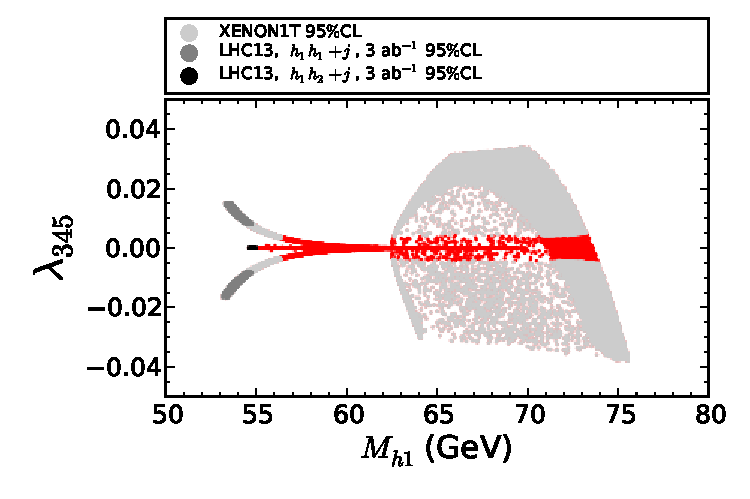
\includegraphics[width=0.5\textwidth]{./Figures/Mh1_ld345_Omega_relic-small-coll_zz-monoc.pdf}%
%  \includegraphics[width=0.5\textwidth]{./Figures/Mh1_Mhc_Omega_relic-small-coll_zz-monoc.pdf}\\
 % 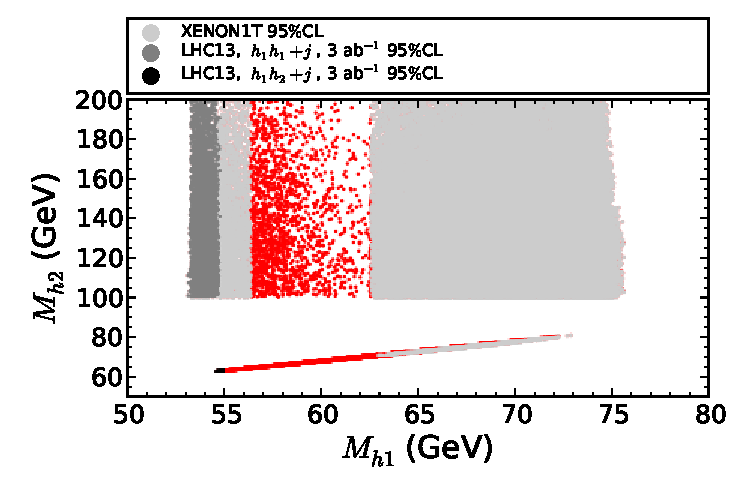
\includegraphics[width=0.5\textwidth]{./Figures/Mh1_Mh2_Omega_relic-small-coll_zz-monoc.pdf}%
%  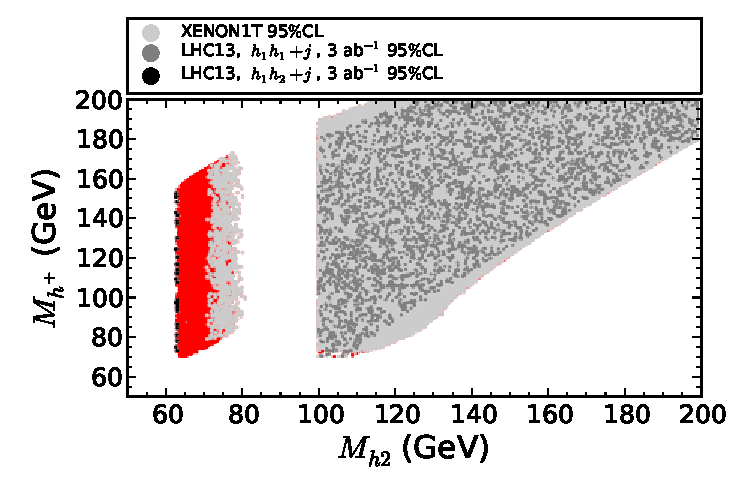
\includegraphics[width=0.5\textwidth]{./Figures/Mhc_Mh2_Omega_relic-small-coll_zz-monoc.pdf}\\
%\caption{}
%\label{}
%\end{figure}
